\section*{Appendix}
\addcontentsline{toc}{section}{Appendix}

\par Here I include the results of the SMM procedure when matching wealth data from different waves of the SCF survey. The general takeaway is that the fit of the model is robust to using different years of wealth data. One notable finding is that, for these later waves of the survey, the lowest estimated point is smaller and the highest estimated point is higher, corresponding with more heterogeneity in returns. 

\section{Results from 2007 wealth data}

\subsection{Estimated distribution of returns}

\par This table provides the results from the four versions of the model (either infinite horizon or life cycle with and without heterogeneity) as described my the mean and standard deviation of the uniform distirbution which makes the simulated wealth moments closest to the wealth moments measured in the 2007 survey.

\begin{center}
    \begin{tabular}{|c|c|c|}
\hline
& Mean & St. Dev \\
\hline
PY-Point & 1.060 & 0.0  \\
PY-Dist & 1.020  &  0.012  \\
LC-Point & 1.043 & 0.0  \\
LC-Dist & .999  &  0.016 \\
\hline
    \end{tabular}
    \end{center}

\subsection{Implied elasticities}

\par Here are the results for the seven estimated points for the discretized uniform distribution and the 7 implied elasticies for each of the variations of the model matching 2007 SCF data. 

\begin{center}
\begin{tabular}{|c|c|c|c|}
\hline
\multicolumn{2}{|c|}{PY} & \multicolumn{2}{|c|}{LC} \\
\hline
Estimated returns & Implied elasticities & Estimated returns & Implied elasticities \\
\hline
0.960 & 7.120 & 0.916 & 5.126 \\
0.980 & 8.518 & 0.944 & 6.253 \\
0.999 & 10.498 & 0.972 & 7.889 \\
1.020 & 13.517 & 0.999 & 10.479 \\
1.039 & 18.688 & 1.027 & 15.197 \\
1.059 & 29.578 & 1.055 & 26.499 \\
1.079 & 67.432 & 1.083 & 90.016 \\
\hline
\end{tabular}
\end{center}


\subsection{Untargeted moments}

\par These three tables present the wealth moments by age cohort for the 2007 wave of the SCF~\ref{fig:EmpLorenzTar2007} , and the simulated version of these untargeted moments for the life cycle version of the model without heterogeneity~\ref{fig:SimLorenzTarPoint2007} and then with heterogeneity~\ref{fig:SimLorenzTarDist2007}.

\begin{figure}[h]
\centering
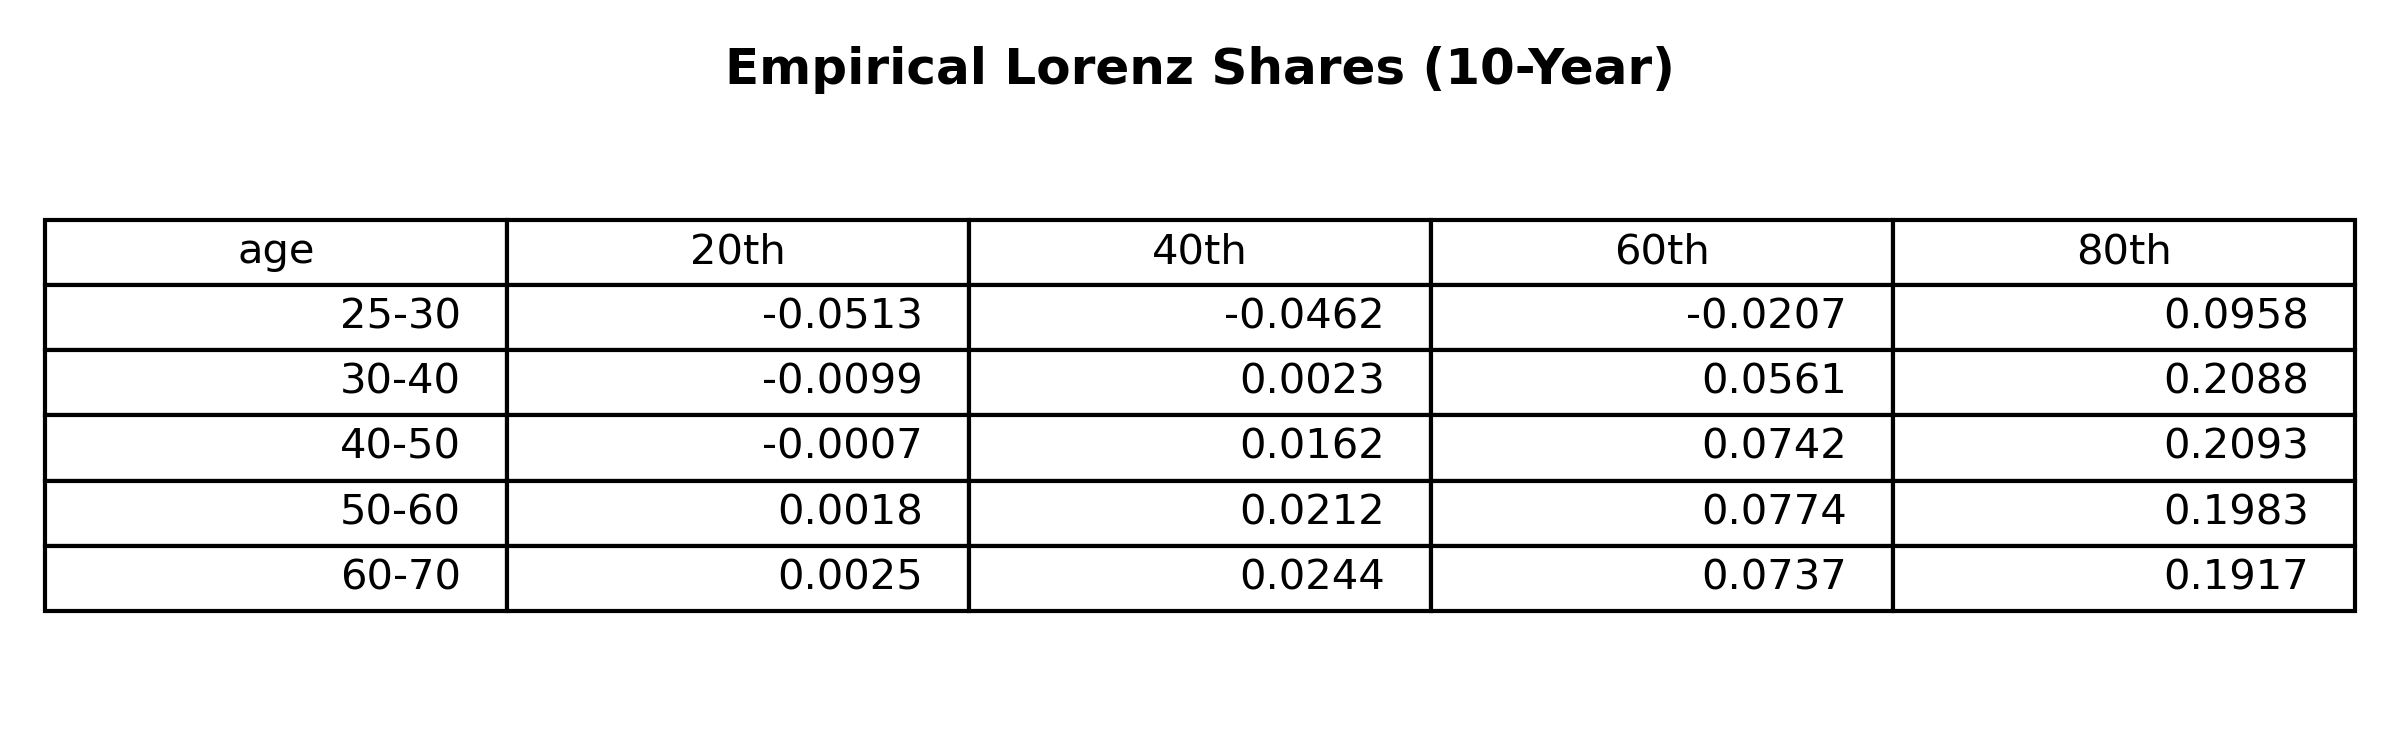
\includegraphics[width=0.8\textwidth]{Tables/Emp_Lorenz_10yr_LCrrDistNetWorth_2007.png}
\caption{Empirical Lorenz Curve Targets from the 2007 SCF.}
\label{fig:EmpLorenzTar2007}
\end{figure}

\begin{figure}[htbp]
\centering
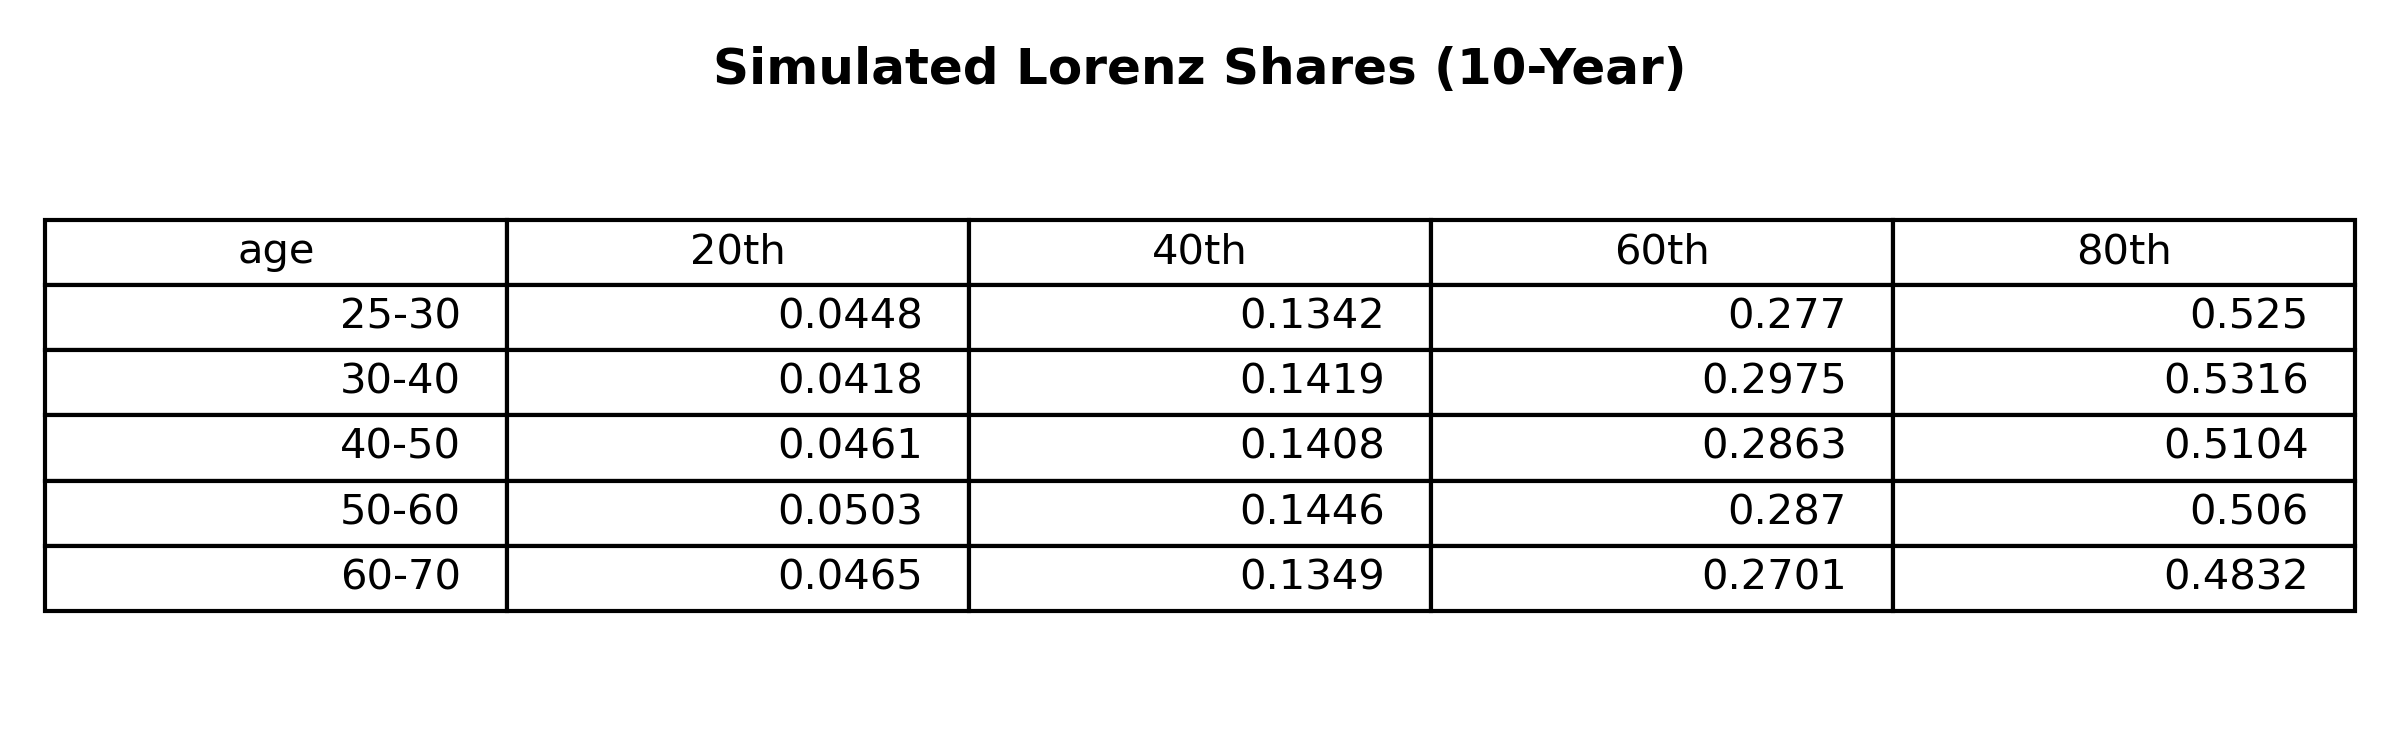
\includegraphics[width=0.8\textwidth]{Tables/Sim_Lorenz_10yr_LCrrPointNetWorth_2007.png}
\caption{Simulated Untargeted Moments without Heterogeneity (R-point).}
\label{fig:SimLorenzTarPoint2007}
\end{figure}

\begin{figure}[htbp]
\centering
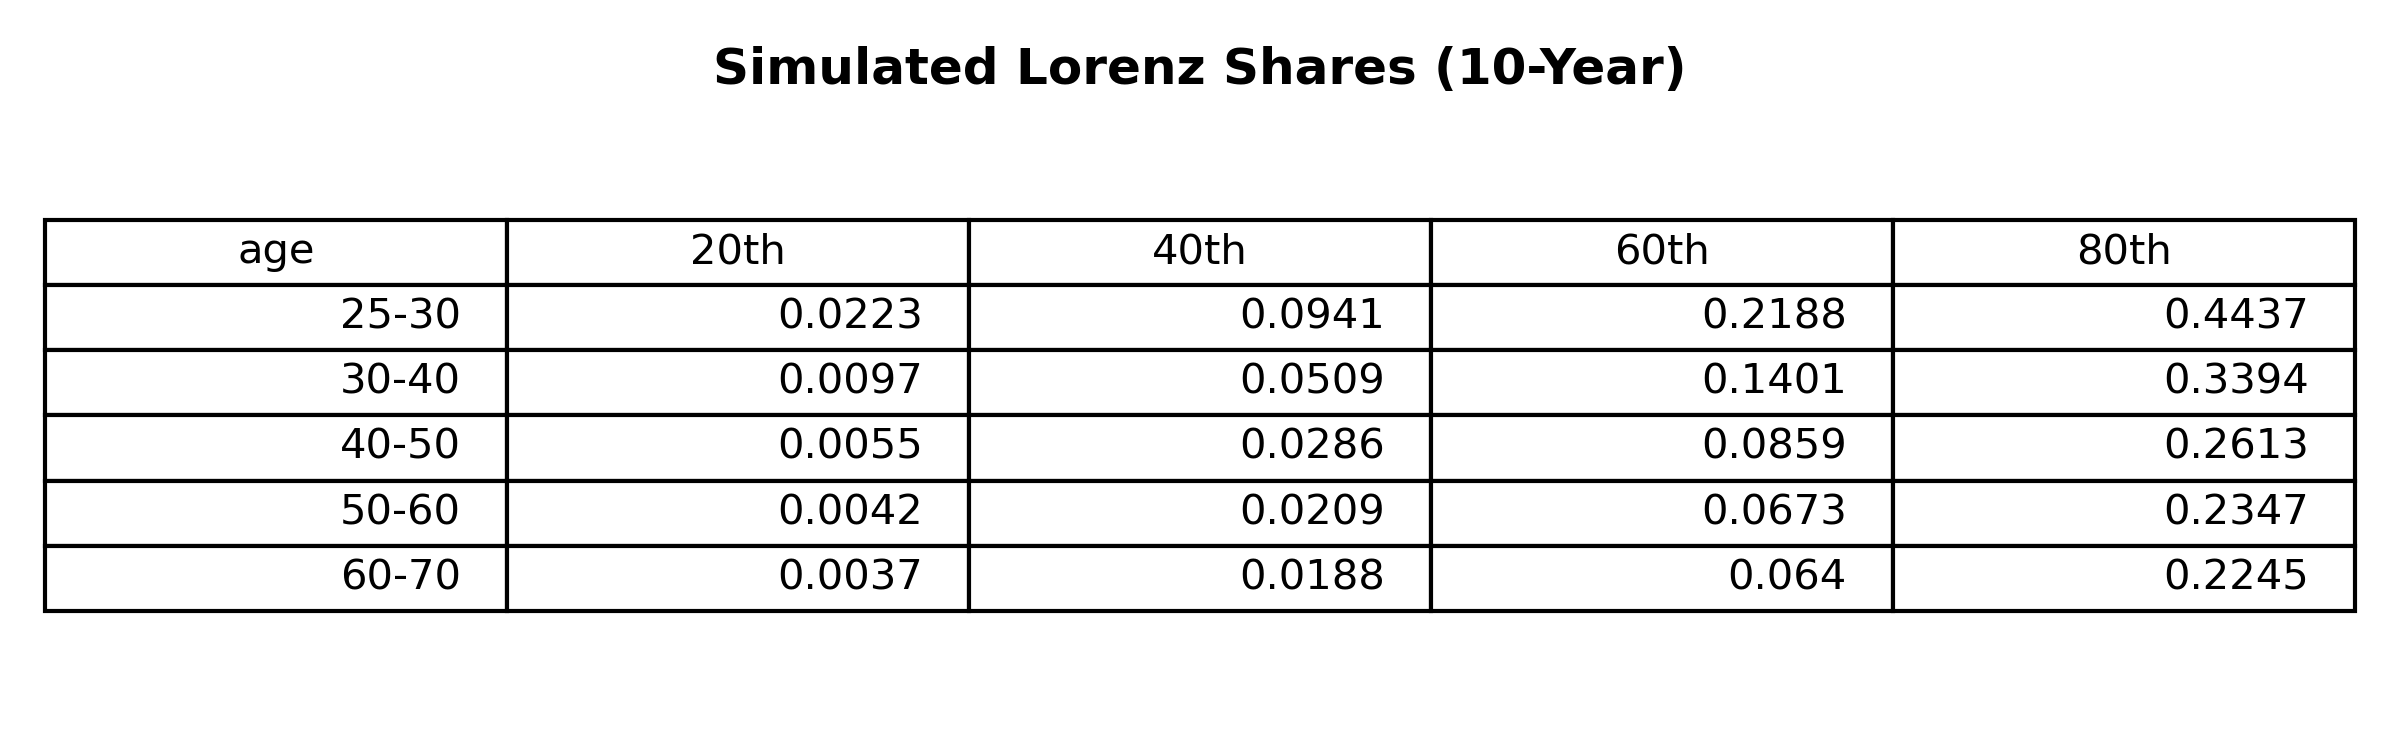
\includegraphics[width=0.8\textwidth]{Tables/Sim_Lorenz_10yr_LCrrDistNetWorth_2007.png}
\caption{Simulated Untargeted Moments with Heterogeneity (R-dist).}
\label{fig:SimLorenzTarDist2007}
\end{figure}

%%%%%%%%%%%%%%%%%%%%%%%%%%%%%%%%%%%%%
\section{Results from 2010 wealth data}

\subsection{Estimated distribution of returns}

\par Here are the results from the four versions of the model  which makes the simulated wealth moments closest to the wealth moments measured in the 2010 survey.

\begin{center}
    \begin{tabular}{|c|c|c|}
\hline
& Mean & St. Dev \\
\hline
PY-Point & 1.060 & 0.0  \\
PY-Dist & 1.002  &  0.015  \\
LC-Point & 1.042 & 0.0  \\
LC-Dist & .981  &  0.020 \\
\hline
    \end{tabular}
    \end{center}

\subsection{Implied elasticities}

\par Here are the results for the seven estimated points for the discretized uniform distribution and the 7 implied elasticies for each of the variations of the model matching 2010 SCF data. 

\begin{center}
\begin{tabular}{|c|c|c|c|}
\hline
\multicolumn{2}{|c|}{PY} & \multicolumn{2}{|c|}{LC} \\
\hline
Estimated returns & Implied elasticities & Estimated returns & Implied elasticities \\
\hline
0.923 & 5.396 & 0.876 & 3.995 \\
0.950 & 6.540 & 0.911 & 4.947 \\
0.976 & 8.184 & 0.946 & 6.347 \\
1.002 & 10.743 & 0.981 & 8.608 \\
1.028 & 15.280 & 1.016 & 12.882 \\
1.054 & 25.531 & 1.051 & 24.002 \\
1.080 & 70.639 & 1.086 & 124.683 \\
\hline
\end{tabular}
\end{center}


\subsection{Untargeted moments}

\par These three tables present the wealth moments by age cohort for the 2010 wave of the SCF~\ref{fig:EmpLorenzTar2010} , and the simulated version of these untargeted moments for the life cycle version of the model without heterogeneity~\ref{fig:SimLorenzTarPoint2010} and then with heterogeneity~\ref{fig:SimLorenzTarDist2010}.

\begin{figure}[h]
\centering
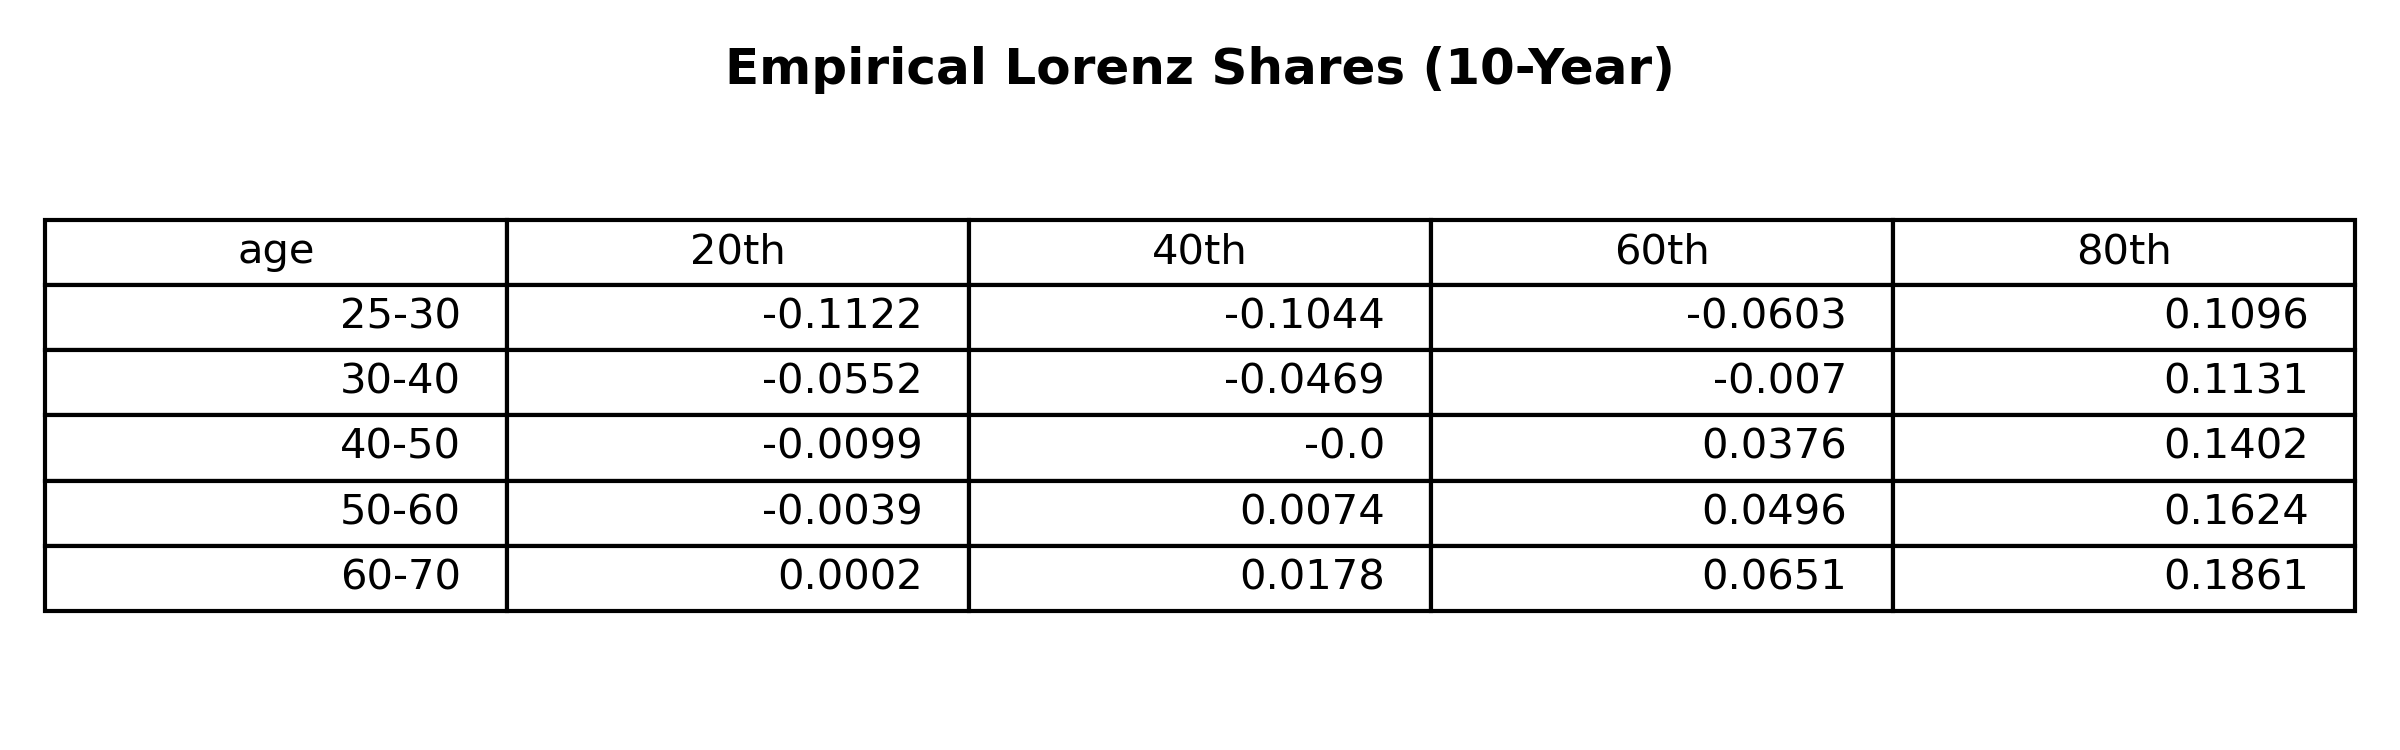
\includegraphics[width=0.8\textwidth]{Tables/Emp_Lorenz_10yr_LCrrDistNetWorth_2010.png}
\caption{Empirical Lorenz Curve Targets from the 2010 SCF.}
\label{fig:EmpLorenzTar2010}
\end{figure}

\begin{figure}[htbp]
\centering
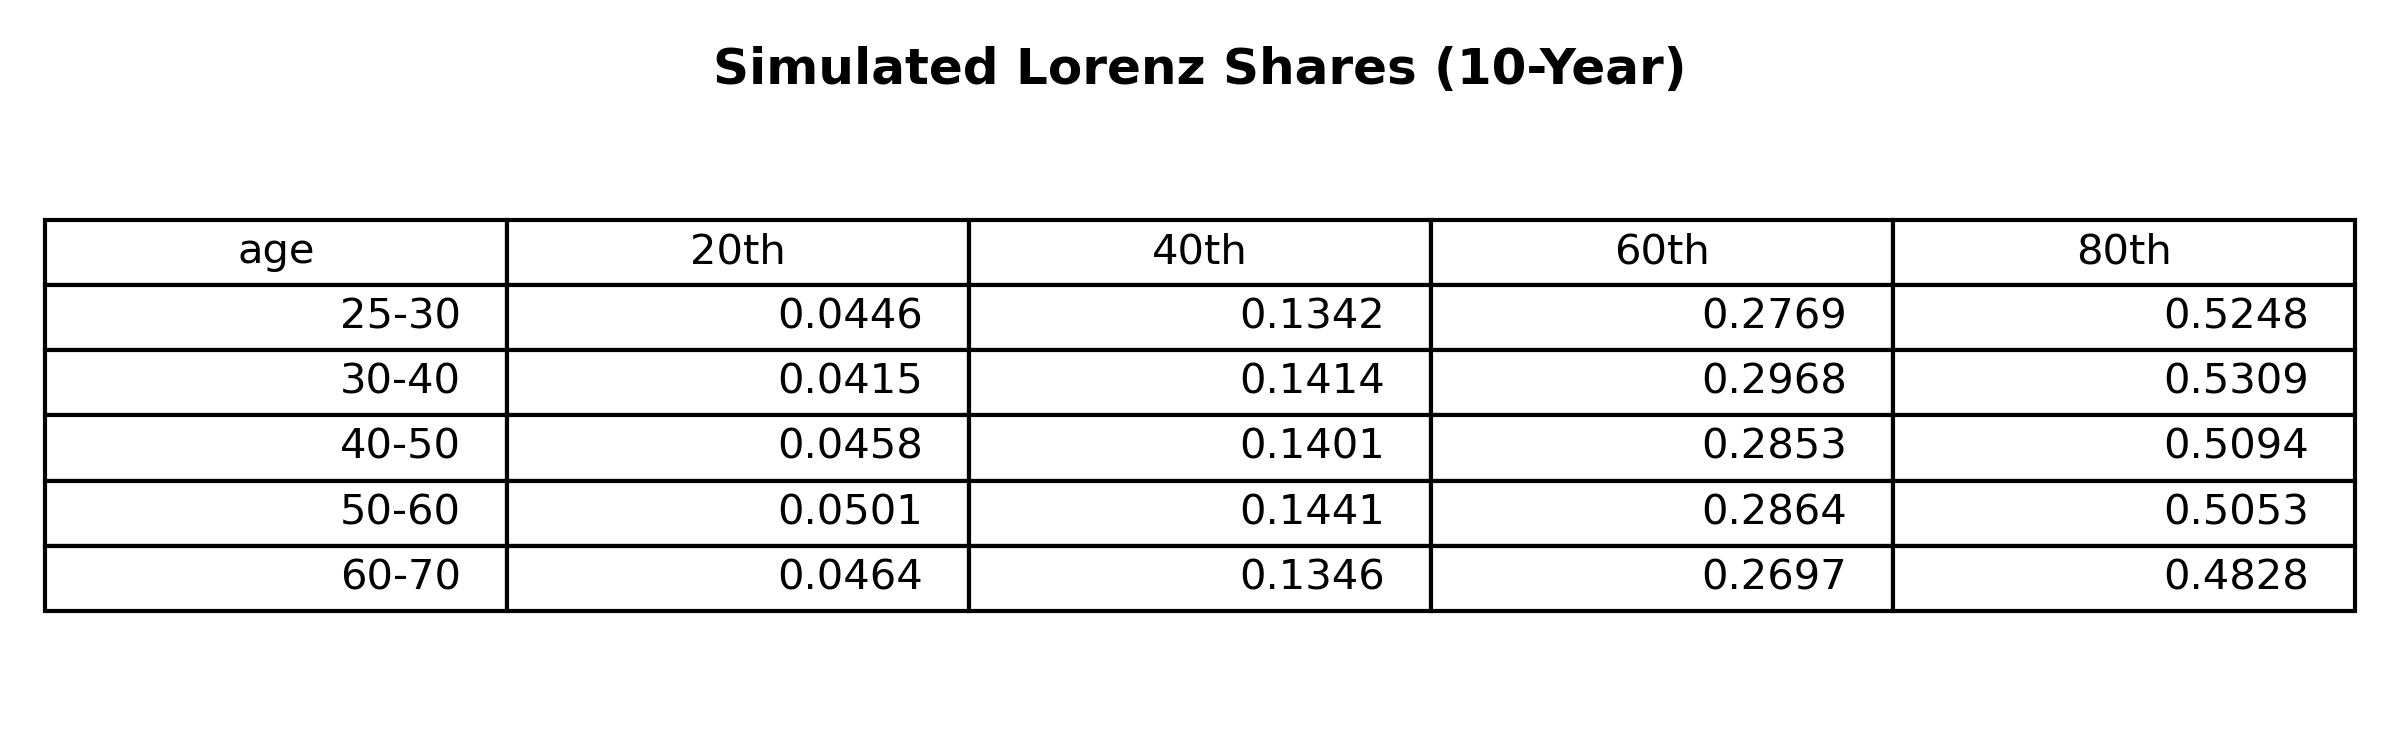
\includegraphics[width=0.8\textwidth]{Tables/Sim_Lorenz_10yr_LCrrPointNetWorth_2010.png}
\caption{Simulated Untargeted Moments without Heterogeneity (R-point).}
\label{fig:SimLorenzTarPoint2010}
\end{figure}

\begin{figure}[htbp]
\centering
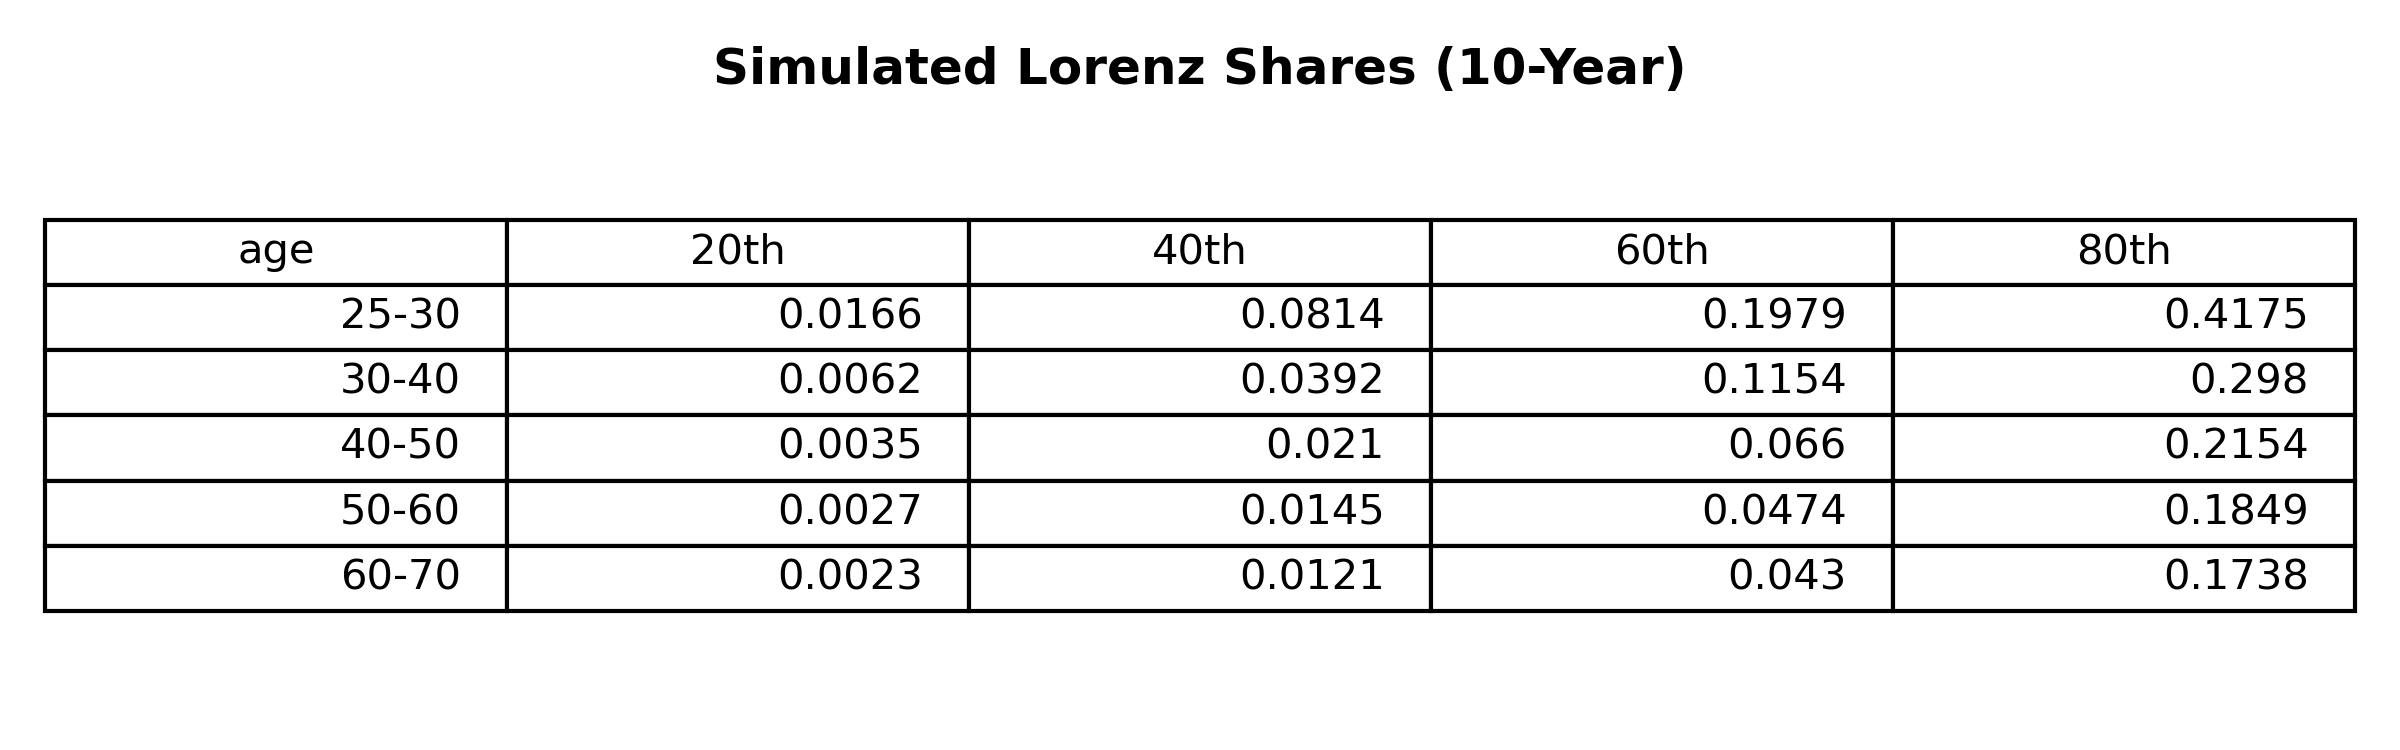
\includegraphics[width=0.8\textwidth]{Tables/Sim_Lorenz_10yr_LCrrDistNetWorth_2010.png}
\caption{Simulated Untargeted Moments with Heterogeneity (R-dist).}
\label{fig:SimLorenzTarDist2010}
\end{figure}


%%%%%%%%%%%%%%%%%%%%%%%%%%%%%%%%%%%%%%
\section{Results from 2013 wealth data}

\subsection{Estimated distribution of returns}

\par Here are the results from the four versions of the model  which makes the simulated wealth moments closest to the wealth moments measured in the 2013 survey.

\begin{center}
    \begin{tabular}{|c|c|c|}
\hline
& Mean & St. Dev \\
\hline
PY-Point & 1.060 & 0.0  \\
PY-Dist & .999  &  0.016  \\
LC-Point & 1.042 & 0.0  \\
LC-Dist & .979  &  0.021 \\
\hline
    \end{tabular}
    \end{center}

\subsection{Implied elasticities}

\par Here are the results for the seven estimated points for the discretized uniform distribution and the 7 implied elasticies for each of the variations of the model matching 2013 SCF data. 

\begin{center}
\begin{tabular}{|c|c|c|c|}
\hline
\multicolumn{2}{|c|}{PY} & \multicolumn{2}{|c|}{LC} \\
\hline
Estimated returns & Implied elasticities & Estimated returns & Implied elasticities \\
\hline
0.920 & 5.263 & 0.872 & 3.911 \\
0.947 & 6.387 & 0.901 & 4.849 \\
0.973 & 8.003 & 0.944 & 6.228 \\
0.999 & 10.524 & 0.979 & 8.460 \\
1.027 & 15.006 & 1.015 & 12.685 \\
1.053 & 25.192 & 1.051 & 23.720 \\
1.080 & 71.032 & 1.086 & 127.148 \\
\hline
\end{tabular}
\end{center}


\subsection{Untargeted moments}

\par These three tables present the wealth moments by age cohort for the 2013 wave of the SCF~\ref{fig:EmpLorenzTar2013} , and the simulated version of these untargeted moments for the life cycle version of the model without heterogeneity~\ref{fig:SimLorenzTarPoint2013} and then with heterogeneity~\ref{fig:SimLorenzTarDist2013}.

\begin{figure}[h]
\centering
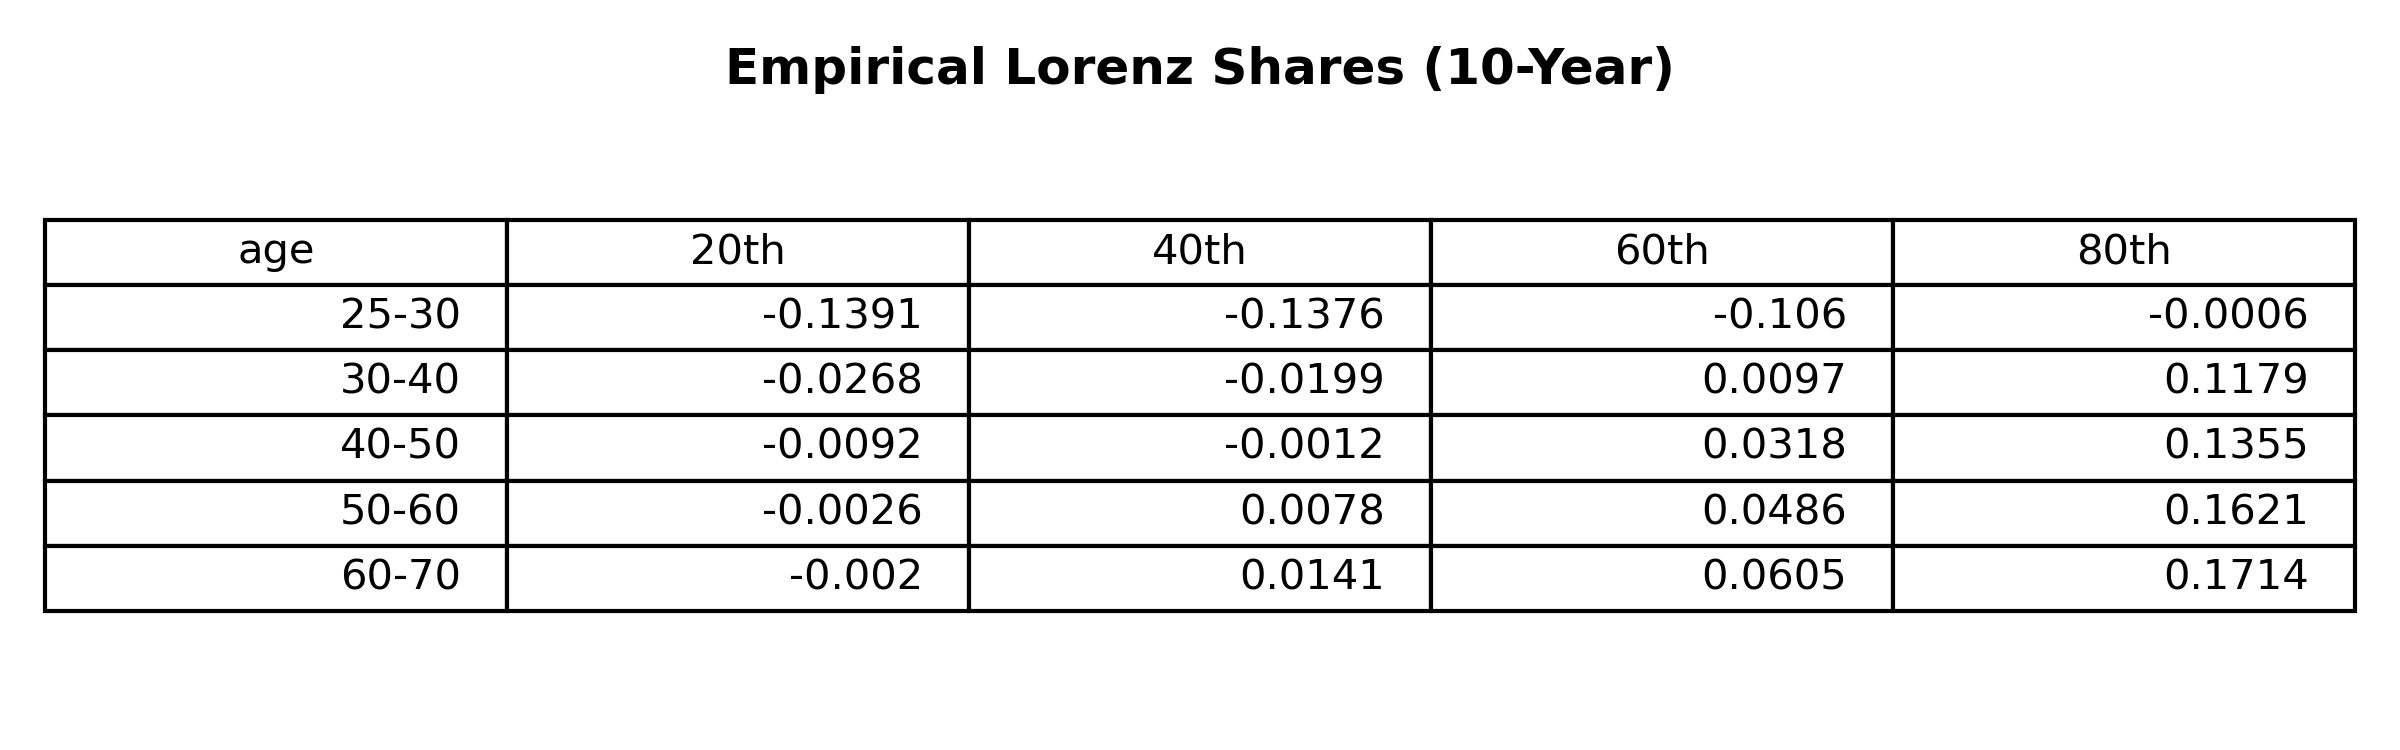
\includegraphics[width=0.8\textwidth]{Tables/Emp_Lorenz_10yr_LCrrDistNetWorth_2013.png}
\caption{Empirical Lorenz Curve Targets from the 2013 SCF.}
\label{fig:EmpLorenzTar2013}
\end{figure}

\begin{figure}[htbp]
\centering
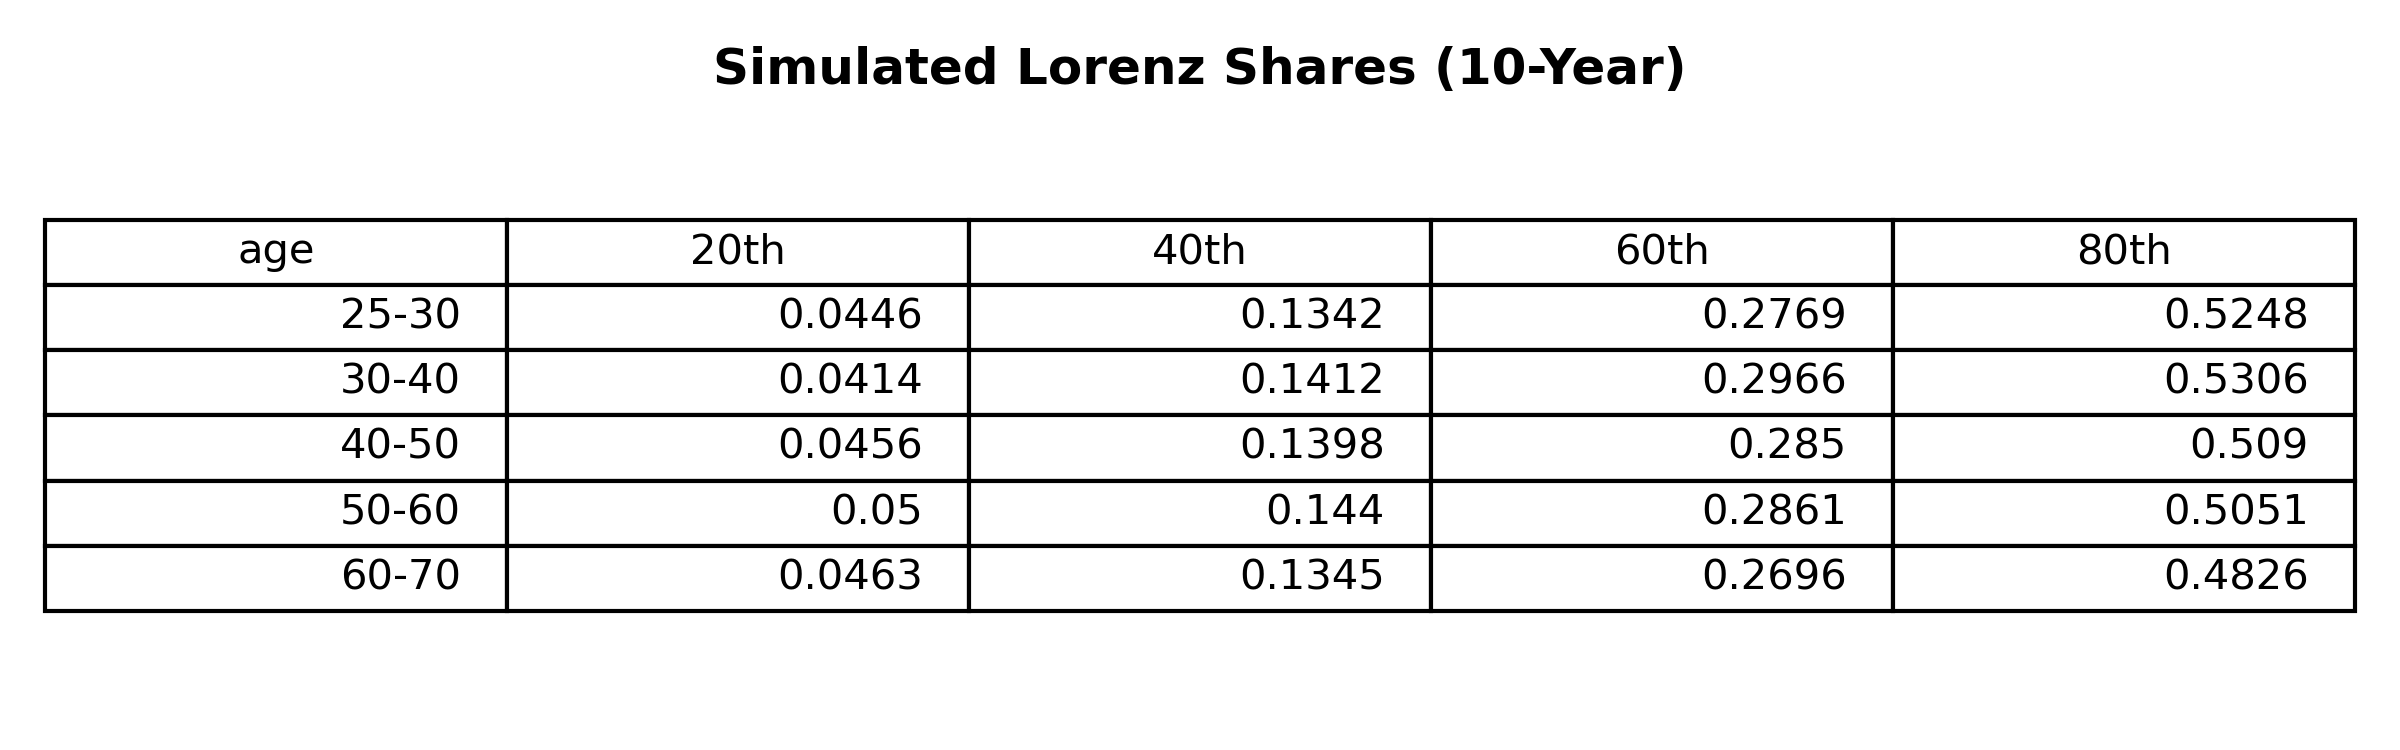
\includegraphics[width=0.8\textwidth]{Tables/Sim_Lorenz_10yr_LCrrPointNetWorth_2013.png}
\caption{Simulated Untargeted Moments without Heterogeneity (R-point).}
\label{fig:SimLorenzTarPoint2013}
\end{figure}

\begin{figure}[htbp]
\centering
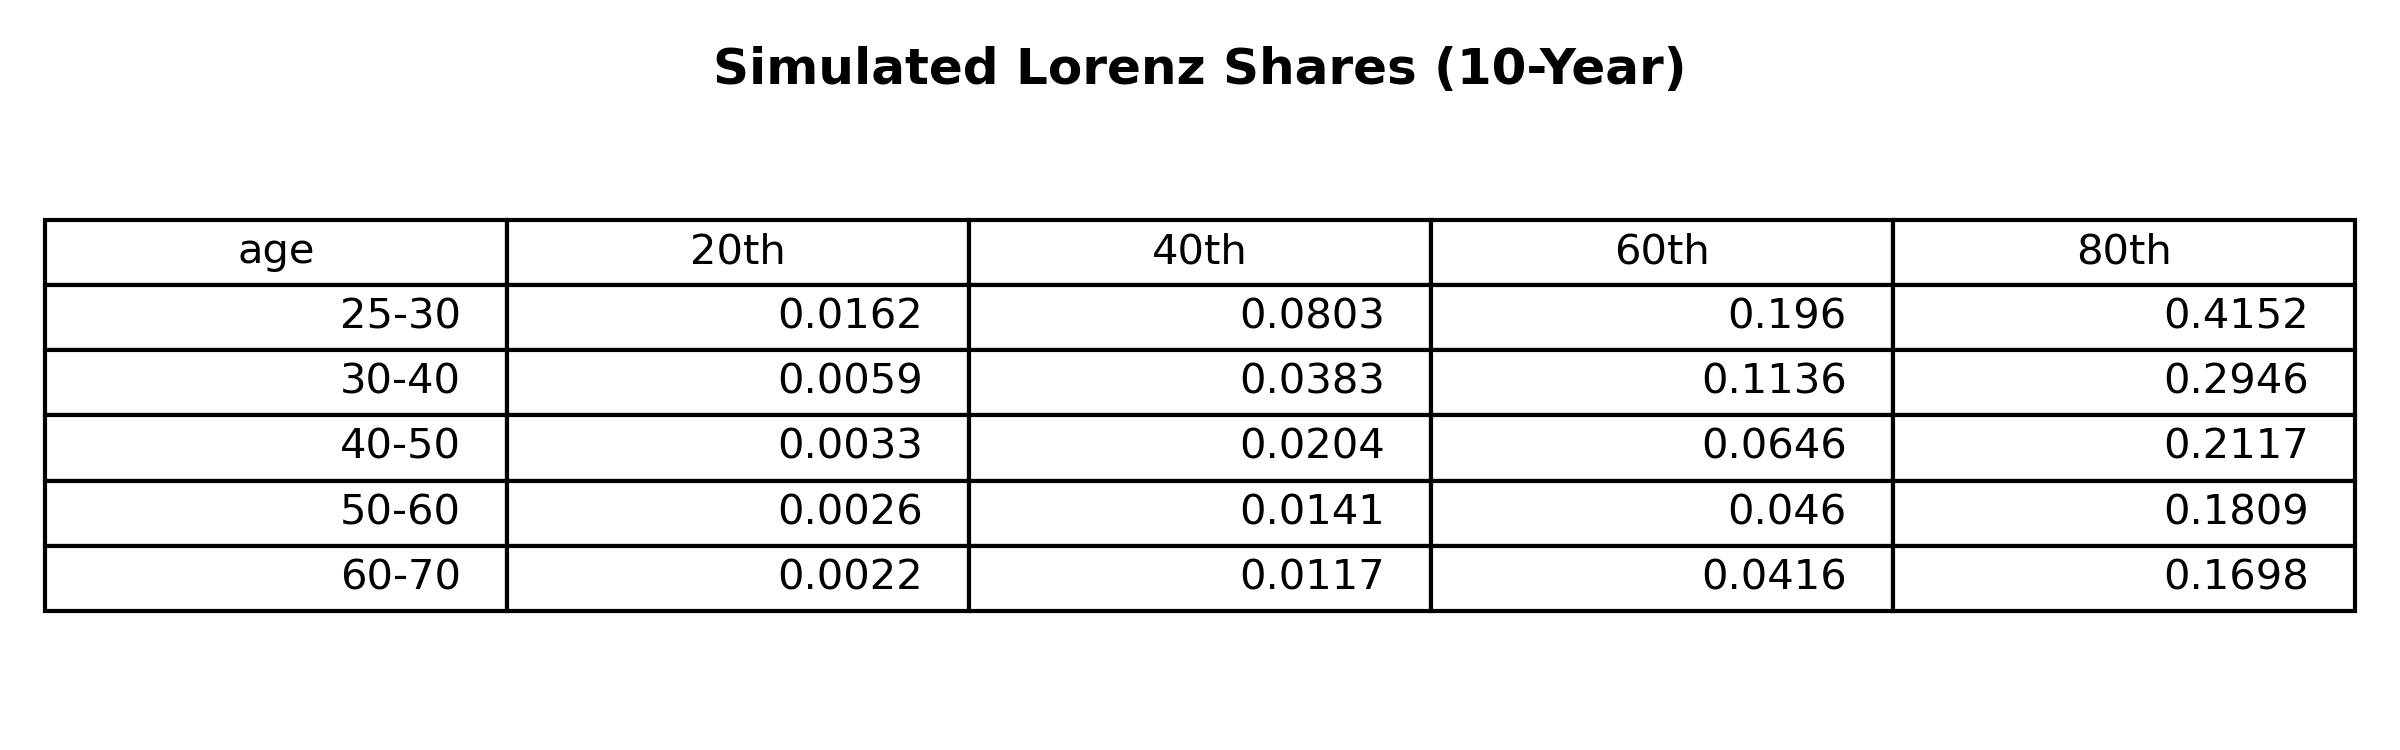
\includegraphics[width=0.8\textwidth]{Tables/Sim_Lorenz_10yr_LCrrDistNetWorth_2013.png}
\caption{Simulated Untargeted Moments with Heterogeneity (R-dist).}
\label{fig:SimLorenzTarDist2013}
\end{figure}

%%%%%%%%%%%%%%%%%%%%%%%%%%%%%%%%%%%%
\section{Results from 2016 wealth data}

\subsection{Estimated distribution of returns}

\par Here are the results from the four versions of the model  which makes the simulated wealth moments closest to the wealth moments measured in the 2016 survey.

\begin{center}
    \begin{tabular}{|c|c|c|}
\hline
& Mean & St. Dev \\
\hline
PY-Point & 1.060 & 0.0  \\
PY-Dist & .993  &  0.017  \\
LC-Point & 1.042 & 0.0  \\
LC-Dist & .972  &  0.023 \\
\hline
    \end{tabular}
    \end{center}

\subsection{Implied elasticities}

\par Here are the results for the seven estimated points for the discretized uniform distribution and the 7 implied elasticies for each of the variations of the model matching 2016 SCF data. 

\begin{center}
\begin{tabular}{|c|c|c|c|}
\hline
\multicolumn{2}{|c|}{PY} & \multicolumn{2}{|c|}{LC} \\
\hline
Estimated returns & Implied elasticities & Estimated returns & Implied elasticities \\
\hline
0.905 & 4.764 & 0.856 & 3.579 \\
0.934 & 5.810 & 0.894 & 4.460 \\
0.963 & 7.319 & 0.933 & 5.762 \\
0.993 & 9.687 & 0.972 & 7.879 \\
1.022 & 13.940 & 1.010 & 11.927 \\
1.051 & 23.816 & 1.049 & 22.755 \\
1.080 & 72.208 & 1.086 & 145.320 \\
\hline
\end{tabular}
\end{center}

\subsection{Untargeted moments}

\par These three tables present the wealth moments by age cohort for the 2016 wave of the SCF~\ref{fig:EmpLorenzTar2016} , and the simulated version of these untargeted moments for the life cycle version of the model without heterogeneity~\ref{fig:SimLorenzTarPoint2016} and then with heterogeneity~\ref{fig:SimLorenzTarDist2016}.

\begin{figure}[h]
\centering
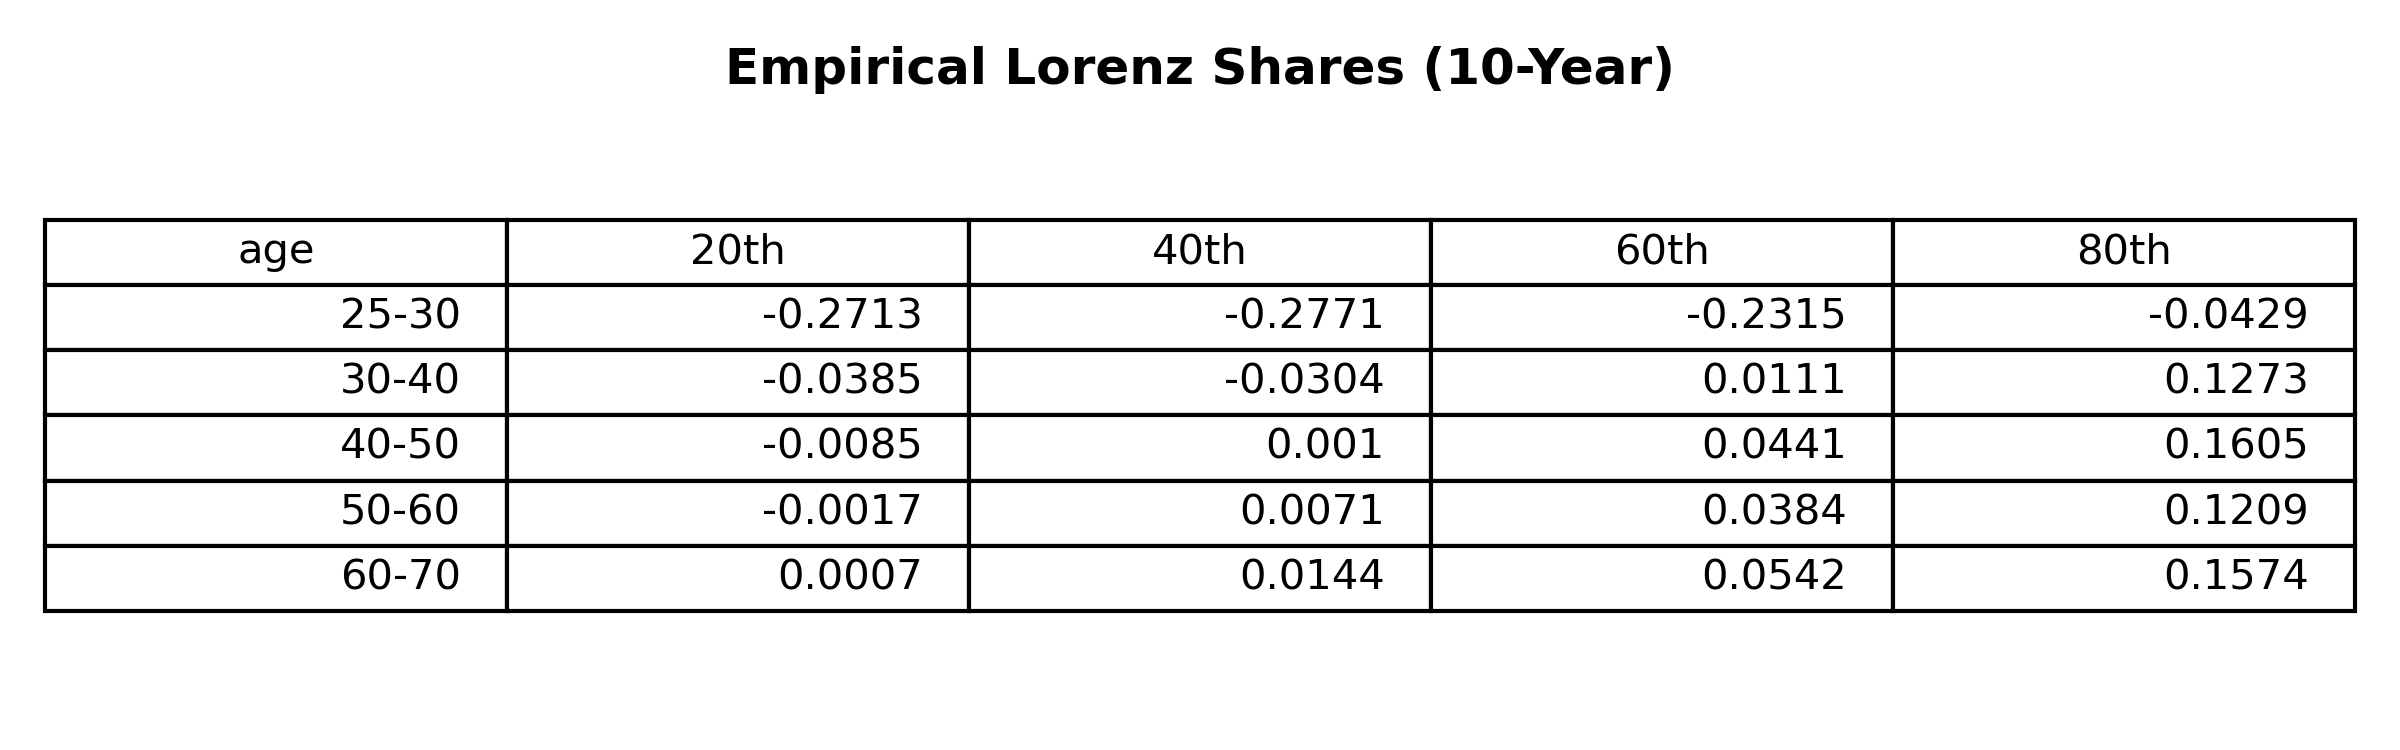
\includegraphics[width=0.8\textwidth]{Tables/Emp_Lorenz_10yr_LCrrDistNetWorth_2016.png}
\caption{Empirical Lorenz Curve Targets from the 2016 SCF.}
\label{fig:EmpLorenzTar2016}
\end{figure}

\begin{figure}[htbp]
\centering
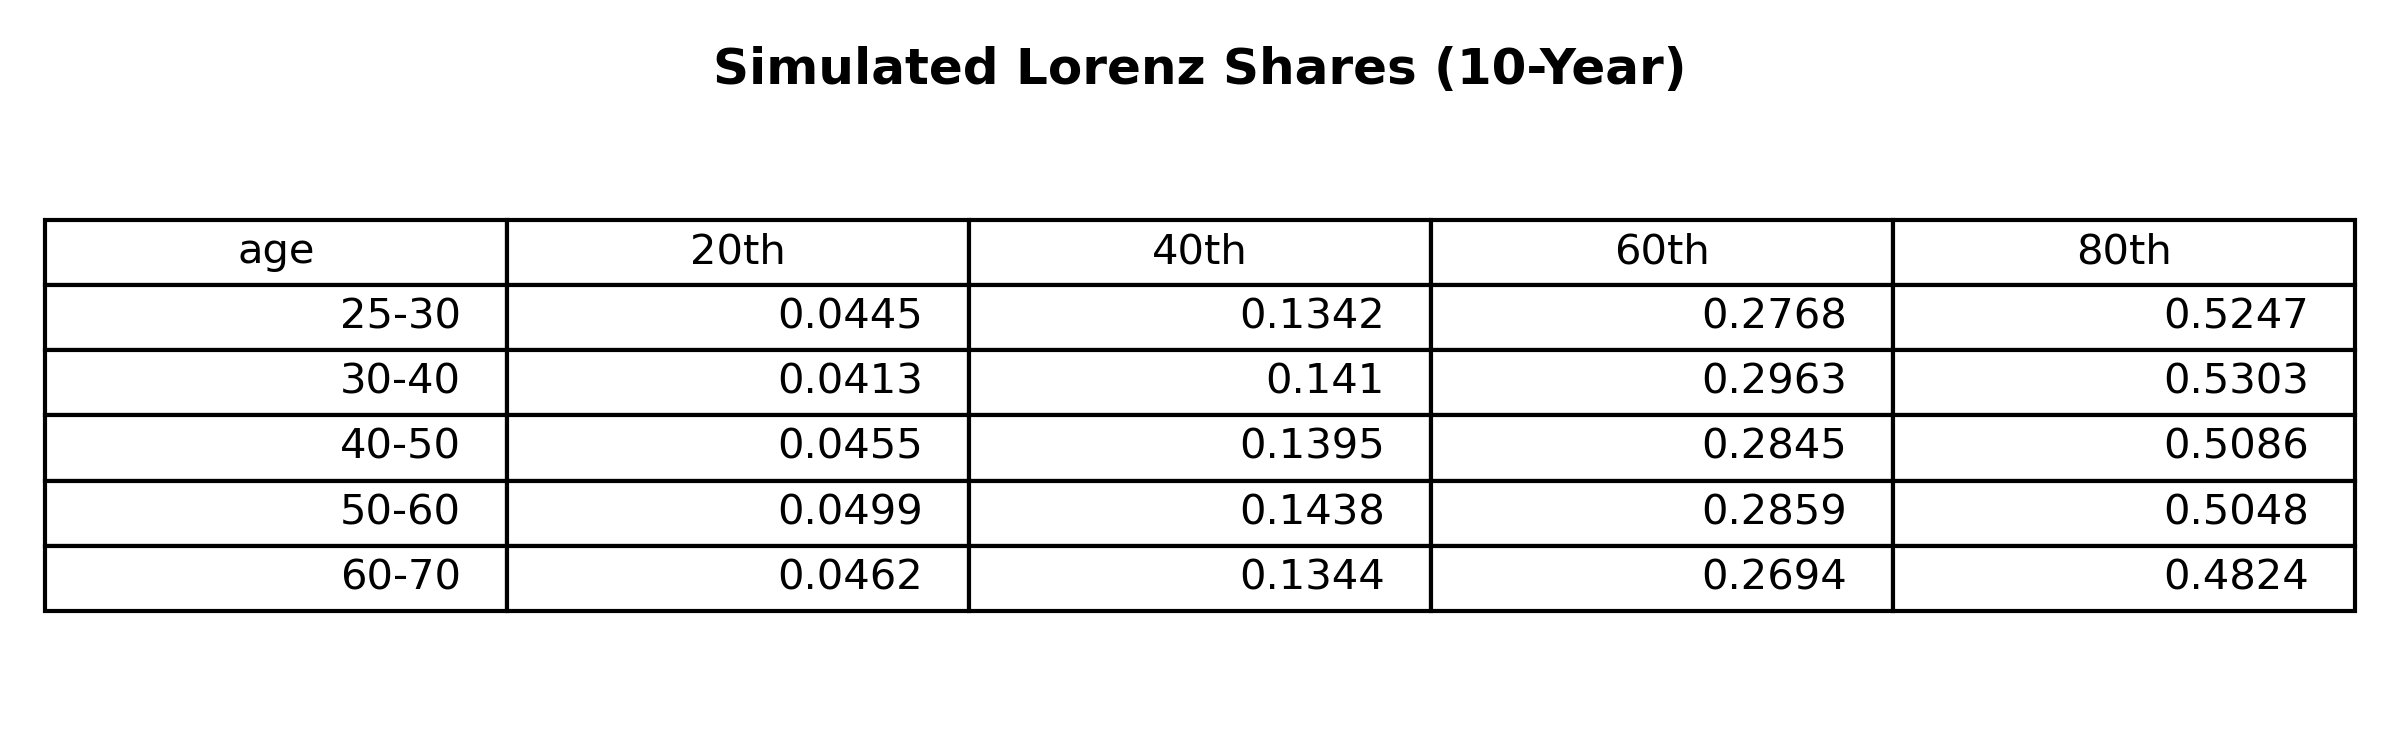
\includegraphics[width=0.8\textwidth]{Tables/Sim_Lorenz_10yr_LCrrPointNetWorth_2016.png}
\caption{Simulated Untargeted Moments without Heterogeneity (R-point).}
\label{fig:SimLorenzTarPoint2016}
\end{figure}

\begin{figure}[htbp]
\centering
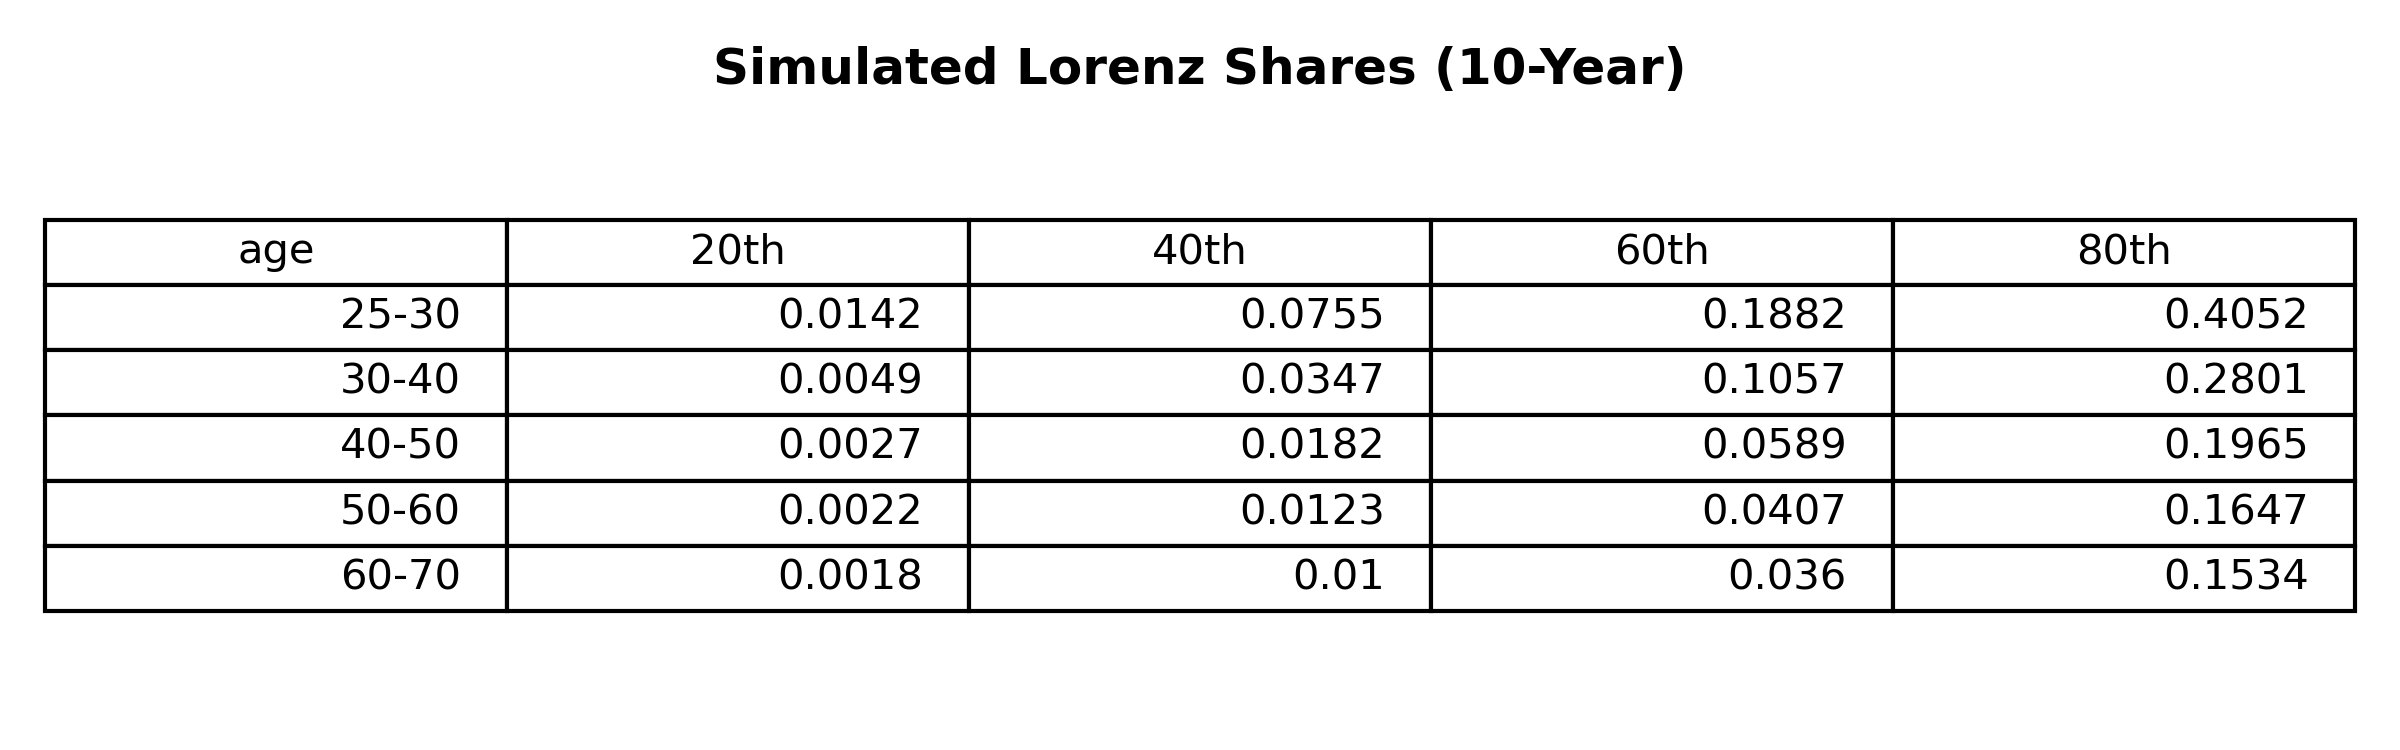
\includegraphics[width=0.8\textwidth]{Tables/Sim_Lorenz_10yr_LCrrDistNetWorth_2016.png}
\caption{Simulated Untargeted Moments with Heterogeneity (R-dist).}
\label{fig:SimLorenzTarDist2016}
\end{figure}

%%%%%%%%%%%%%%%%%%%%%%%%%%%%%%%%%%%%%%%
\section{Results from 2019 wealth data}

\subsection{Estimated distribution of returns}

\par Here are the results from the four versions of the model  which makes the simulated wealth moments closest to the wealth moments measured in the 2019 survey.

\begin{center}
    \begin{tabular}{|c|c|c|}
\hline
& Mean & St. Dev \\
\hline
PY-Point & 1.060 & 0.0  \\
PY-Dist & .999  &  0.016  \\
LC-Point & 1.042 & 0.0  \\
LC-Dist & .978  &  0.021 \\
\hline
    \end{tabular}
    \end{center}

\subsection{Implied elasticities}
    
\par Here are the results for the seven estimated points for the discretized uniform distribution and the 7 implied elasticies for each of the variations of the model matching 2019 SCF data. 

\begin{center}
\begin{tabular}{|c|c|c|c|}
\hline
\multicolumn{2}{|c|}{PY} & \multicolumn{2}{|c|}{LC} \\
\hline
Estimated returns & Implied elasticities & Estimated returns & Implied elasticities \\
\hline
0.923 & 5.204 & 0.876 & 3.868 \\
0.950 & 6.319 & 0.911 & 4.796 \\
0.976 & 7.923 & 0.946 & 6.161 \\
1.002 & 10.426 & 0.981 & 8.369 \\
1.028 & 14.882 & 1.016 & 12.544 \\
1.054 & 25.035 & 1.051 & 23.430 \\
1.080 & 71.174 & 1.086 & 123.510 \\
\hline
\end{tabular}
\end{center}

\subsection{Untargeted moments}

\par These three tables present the wealth moments by age cohort for the 2019 wave of the SCF~\ref{fig:EmpLorenzTar2019} , and the simulated version of these untargeted moments for the life cycle version of the model without heterogeneity~\ref{fig:SimLorenzTarPoint2019} and then with heterogeneity~\ref{fig:SimLorenzTarDist2019}.

\begin{figure}[h]
\centering
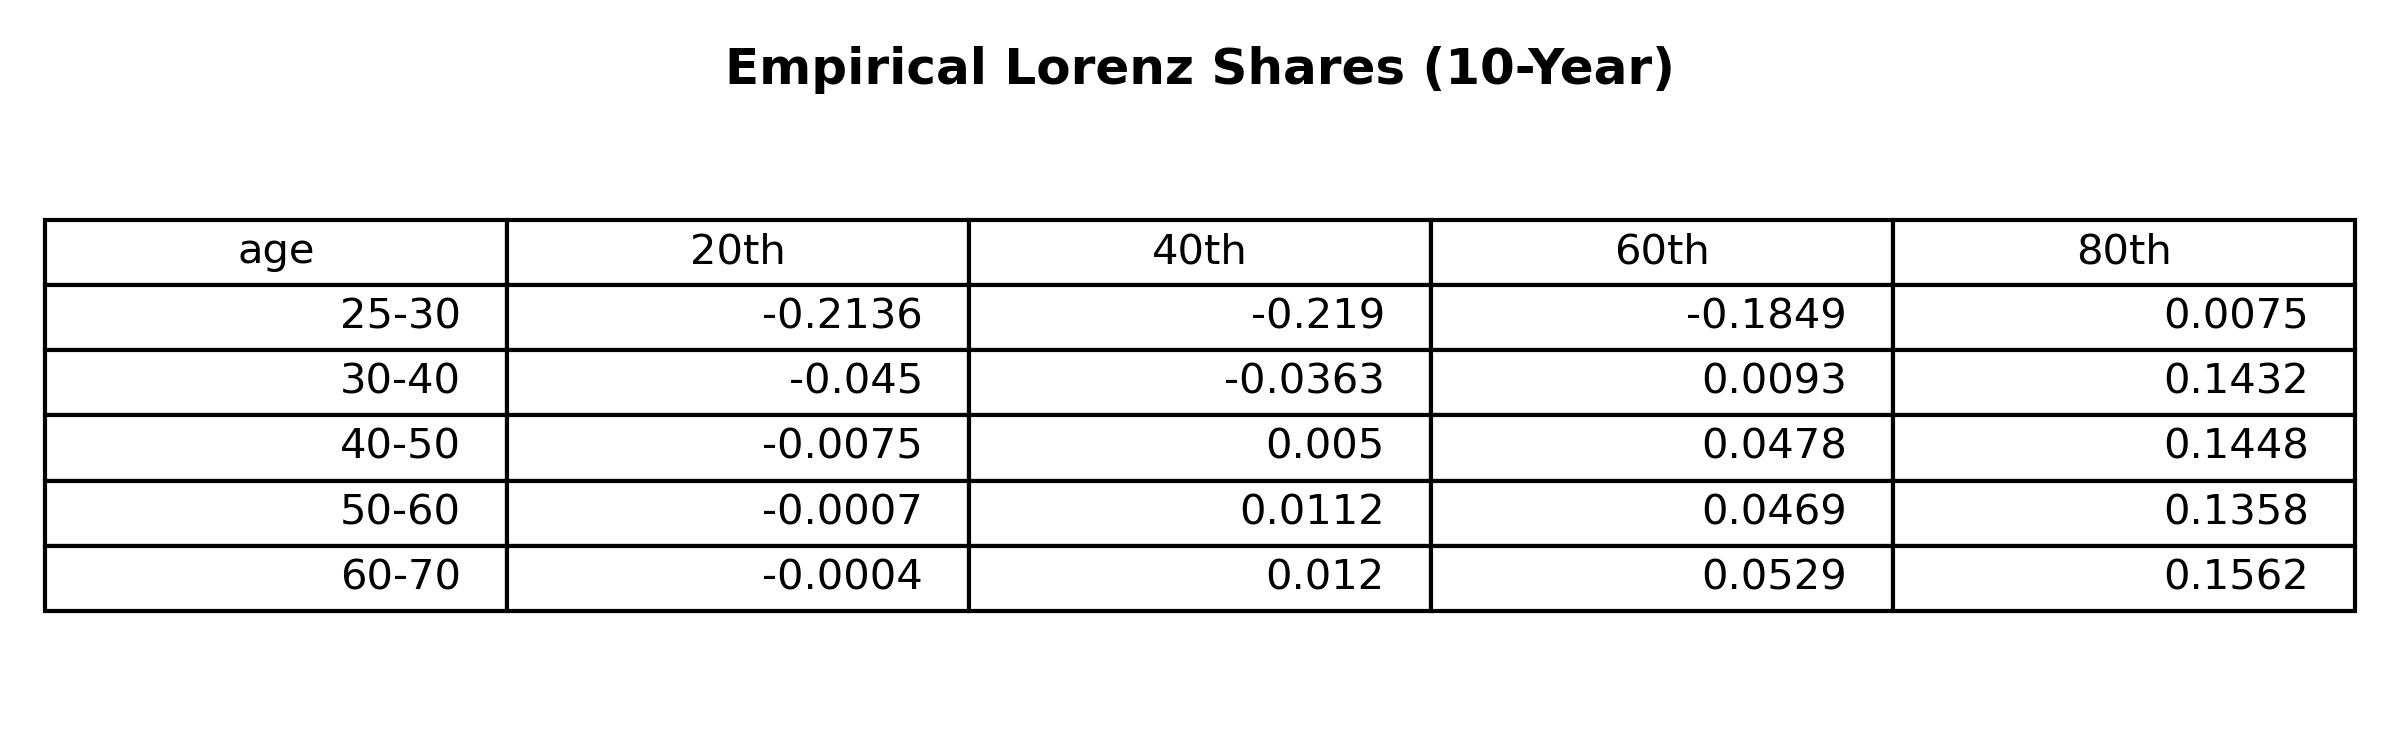
\includegraphics[width=0.8\textwidth]{Tables/Emp_Lorenz_10yr_LCrrDistNetWorth_2019.png}
\caption{Empirical Lorenz Curve Targets from the 2019 SCF.}
\label{fig:EmpLorenzTar2019}
\end{figure}

\begin{figure}[htbp]
\centering
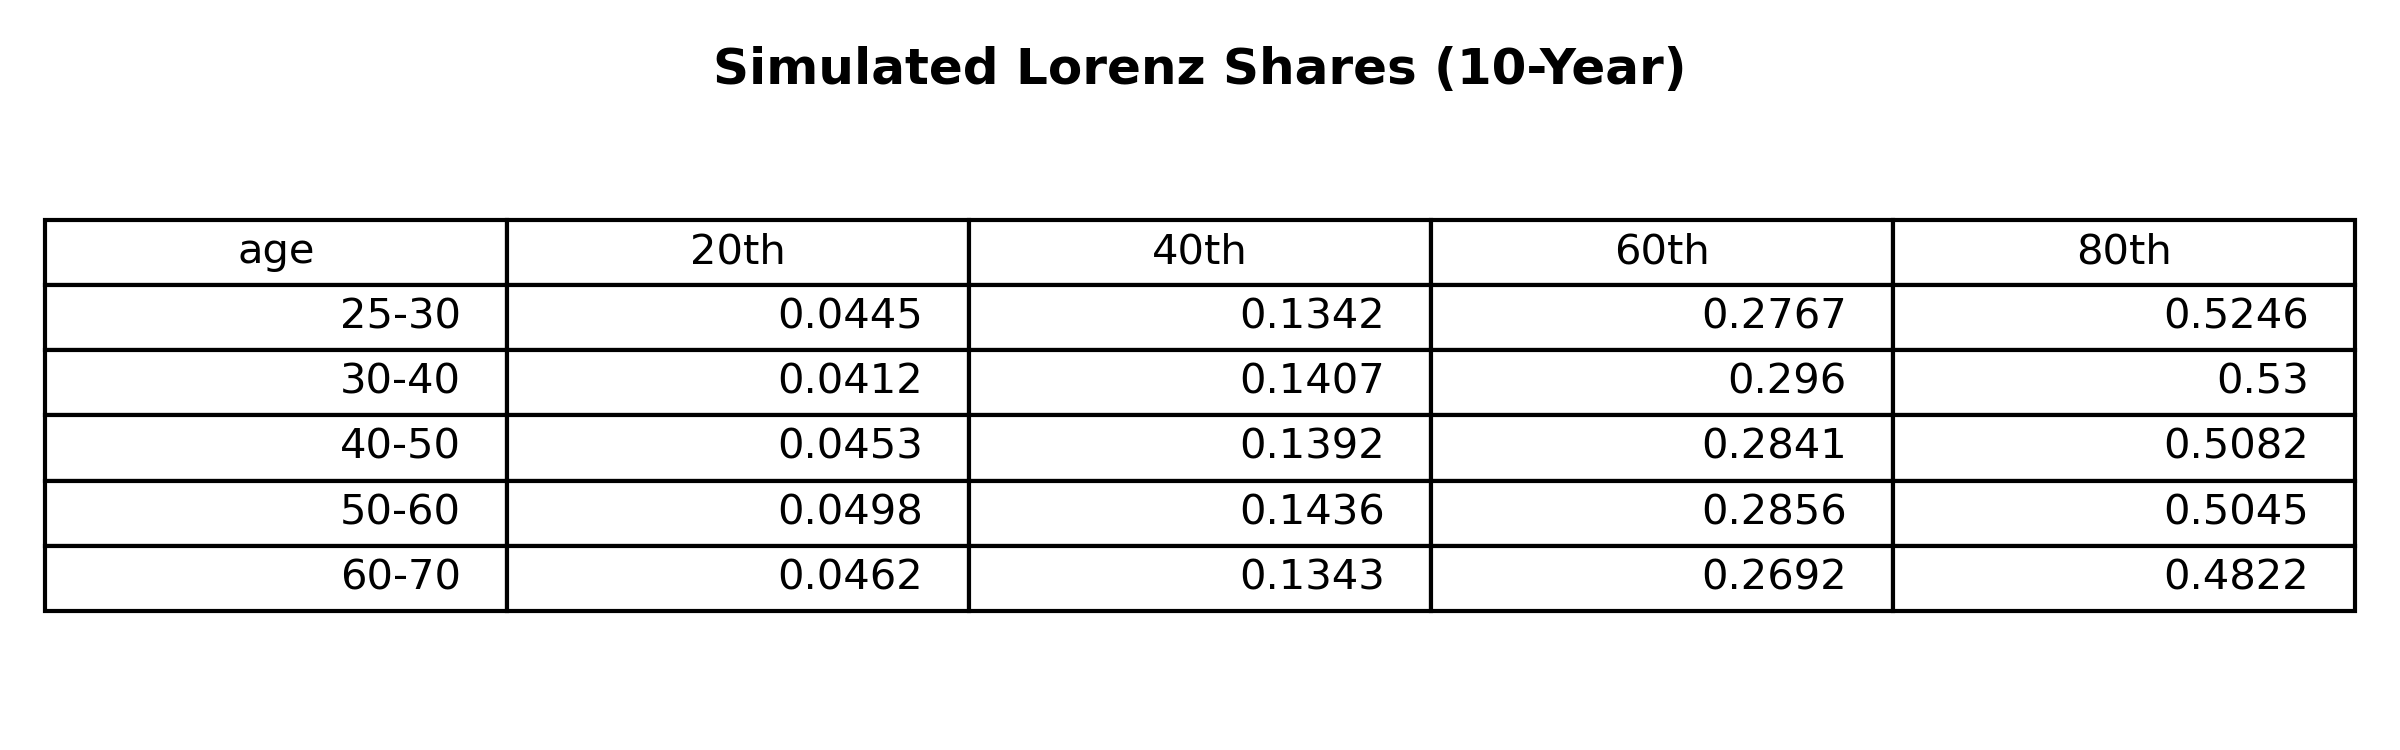
\includegraphics[width=0.8\textwidth]{Tables/Sim_Lorenz_10yr_LCrrPointNetWorth_2019.png}
\caption{Simulated Untargeted Moments without Heterogeneity (R-point).}
\label{fig:SimLorenzTarPoint2019}
\end{figure}

\begin{figure}[htbp]
\centering
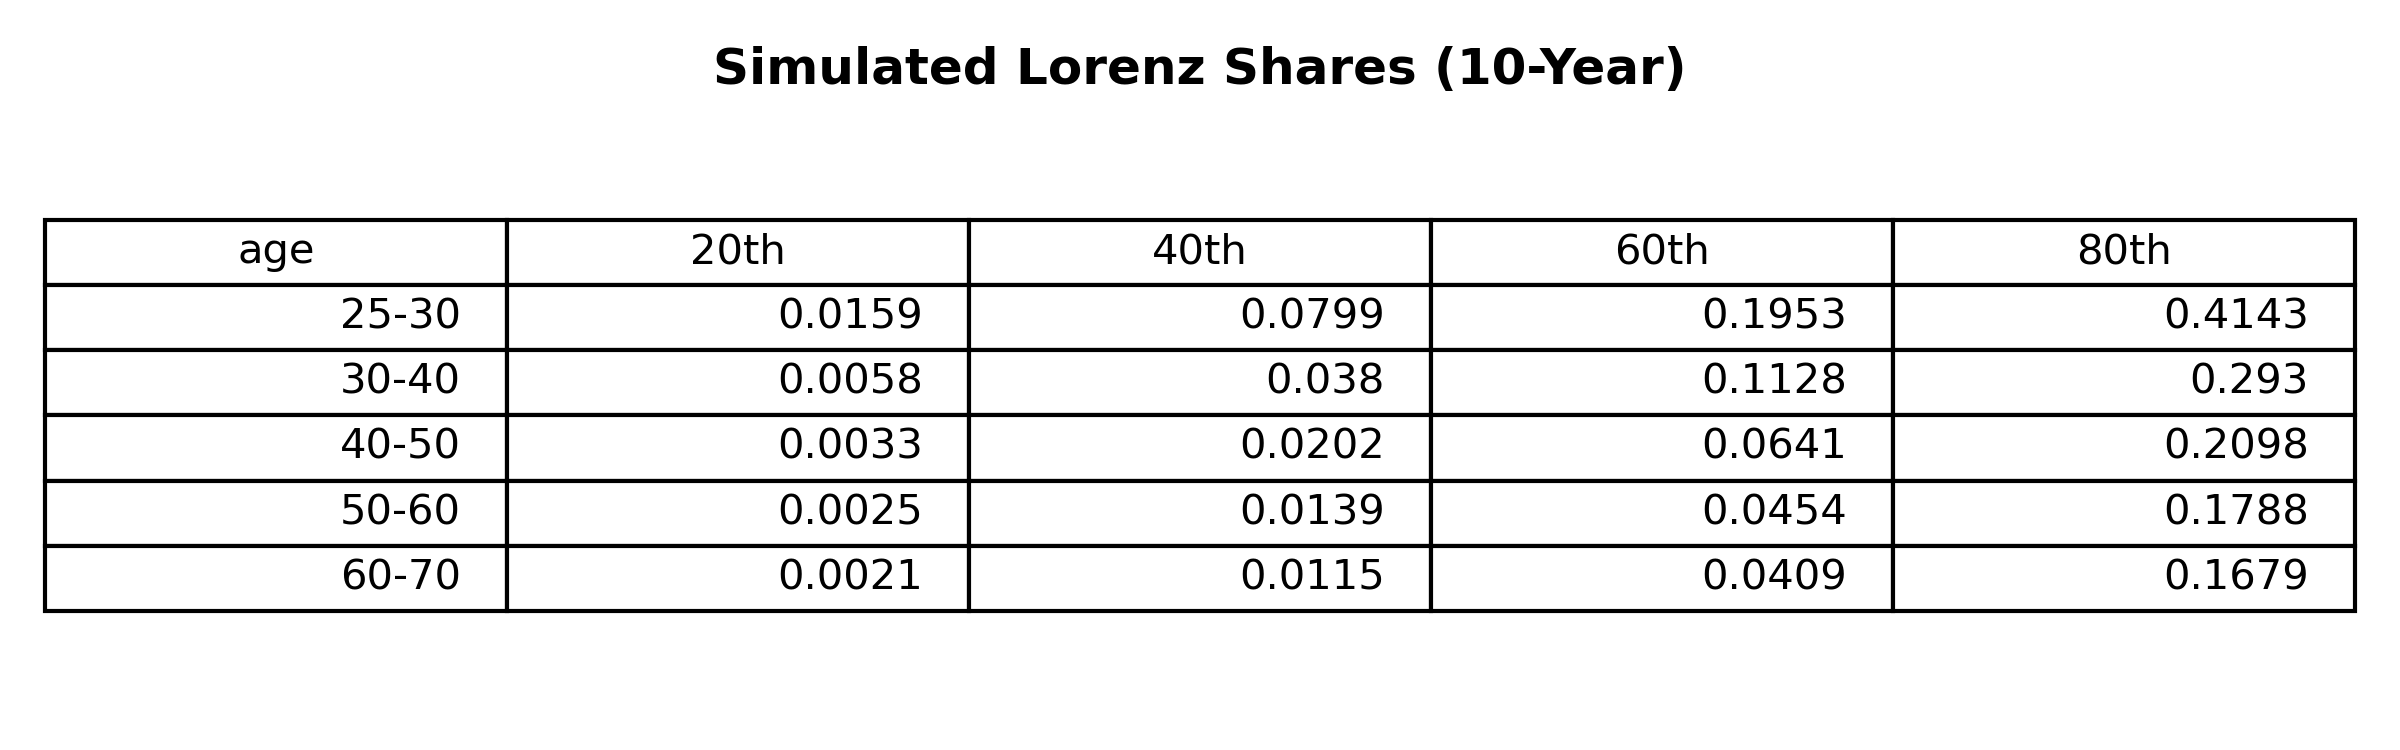
\includegraphics[width=0.8\textwidth]{Tables/Sim_Lorenz_10yr_LCrrDistNetWorth_2019.png}
\caption{Simulated Untargeted Moments with Heterogeneity (R-dist).}
\label{fig:SimLorenzTarDist2019}
\end{figure}
